% Created 2021-10-21 Thu 12:42
% Intended LaTeX compiler: pdflatex
\documentclass[11pt]{article}
\usepackage[utf8]{inputenc}
\usepackage[T1]{fontenc}
\usepackage{graphicx}
\usepackage{grffile}
\usepackage{longtable}
\usepackage{wrapfig}
\usepackage{rotating}
\usepackage[normalem]{ulem}
\usepackage{amsmath}
\usepackage{textcomp}
\usepackage{amssymb}
\usepackage{capt-of}
\usepackage{hyperref}
\author{LiquidZulu}
\date{\today}
\title{Don't Be A Neo-Prag | These People Are Destroying Libertarianism | The Mises Caucus Lost Its Way | The Anti-Liberty Infestation In Our Movement | The Problem With Twitter Ancaps}
\hypersetup{
 pdfauthor={LiquidZulu},
 pdftitle={Don't Be A Neo-Prag | These People Are Destroying Libertarianism | The Mises Caucus Lost Its Way | The Anti-Liberty Infestation In Our Movement | The Problem With Twitter Ancaps},
 pdfkeywords={},
 pdfsubject={},
 pdfcreator={Emacs 27.1 (Org mode 9.5)}, 
 pdflang={English}}
\begin{document}

\maketitle
\tableofcontents


\section{The Purpose of the Mises Caucus}
\label{sec:org537fe76}
The Libertarian Party Mises Caucus was founded for the purpose of principled messaging over pragmatism.\footnote{\url{https://lpmisescaucus.com/platform/}, \emph{Plank 1 --- Property Rights}, ``We condemn all fraud and initiatory violence towards a person’s life, liberty, and property.'' (\href{https://archive.ph/5upKF}{archived})} In interviews Heise is quick to promote his caucus as being a re-ignition of the Ron Paul revolution, the revolution that was built on the premise of reaching the remnant, which in short requires you to focus on principled messaging, and if you are not familiar with that these two videos\footnote{Drew Hancock, ``The Libertarian Case for Radical Messaging,'' \url{https://www.youtube.com/watch?v=Y6qUiD5sAkA}}\textsuperscript{,}\,\footnote{Drew Hancock, ``Reach the Remnant,'' \url{https://www.youtube.com/watch?v=EhEAQCsSFfU}} by Drew Hancock explain the concept in detail.

It was necessary to form this principled caucus because for many years the LP had been under the control of the prag caucus, who were willing to sacrifice the message for the sake of mainstream appeal, citing this as the more ``pragmatic'' approach to achieving liberty. A similar cancer has now gripped the Mises Caucus itself, and if it is not rooted out it could set back the liberty movement by years. This cancer is that of the neo-prags who wish to sacrifice adherence to libertarian ethics out of high time preference\footnote{See @ReadingMises, \url{https://twitter.com/ReadingMises/status/1448936188929249299?s=20}, for more on this.} and frustration with the Cathedral. This is the most urgent problem in intralibertarian discourse. Whether or not it is addressed will determine whether the movement will be characterised by the principles of liberty or impulsive reactions against whatever the enemy does.

\section{Counter Mandates}
\label{sec:org3fa1372}
The most common place where these neo-prags detract from libertarianism is in their desire for various government counter-mandates. You will often see them calling for the state to ban private businesses from rejecting the unvaccinated or alternatively the unmasked. A parallel can be drawn between this and the anti-discrimination laws implemented in the wake of the civil rights movement.

Their general speil is that while not ethical to ban businesses from enforcing that you wear a mask or take a vax, this will be a strike against the Cathedral and as such it will benifit liberty in the long run. We can put our selves in the shoes of civil rights advocates in the US in the 60's and use this logic to justify those anti-discrimination laws too. The Cathedral at that time was no doubt anti-black, and as such forcing businesses to not have private Jim Crow would be an equal strike against it as is forcing businesses to not have private vax or mask mandates.

We can expand this analogy by supposing that the federal government mandated that all businesses must enforce Jim Crow, would the proper libertarian response be to support states enforcing that no business can enforce Jim Crow? That hardly seems right, libertarianism is opposed to all forms of anti-discrimination legislation,\footnote{See Michael Moreno, ``Why the Supreme Court's LGBTQ Ruling Is Immoral,'' \url{https://www.youtube.com/watch?v=KBlf9ubN5jk}, for more on this.} but this is not only an issue of ethics. Expanding the states ability to regulate freedom of association is a terrible strategy for attaining anarchy. If it is possible for states to implement their own mandates why not just negate the federal mandates, rather than negating them \emph{and} implementing their own mandates on top. This is analogous to Walter Blocks framing of abortion as being evicting \emph{and} killing. We can be for the negating of the federal mandate and against the implementation of a state mandate on top of that.

\section{The Hubris of Pragmatism}
\label{sec:org14af6b5}
The neo-prag belief that they know when we should go about expanding the state, and moreover, when they can discount ethics ties into the hubris of pragmatism. But before I elaborate on that I ask that you click the like button if you are also concerned with protecting the liberty movement from subversion.

So, this is a similar concept to what Jordan Peterson speaks of when he discusses the narcissism of authoritarianism. Essentially when I am saying that some previous regime was not real socialism, and that my ideas could implement proper socialism, what I am really saying is that I am smarter than those previous dictators and that if I was the dictator I could do a better job. A similar thing happens when I say that I can decide when ethics apply and when they don't; in saying that I imply that I am smarter than everyone else. How so? You may be asking, this is because of a second premise they take up, that they don't want others to decide when ethics dont apply to them. This is the essence of libertarianism, and these people still consider themselves libertarian, the belief that a person or a group of people are capable and that they should centrally plan ethics in this manner is statism. And as these people are at least ostensibly anarchist, what they are saying is that statism is fine so long as they are in charge.

\section{Walk Away From Omelas}
\label{sec:org14c5852}
If you are not like that and wish to actually remain consistent in your principles a good test of that is found in the short story ``The Ones Who Walk Away from Omelas.'' The story is about a perfect utopia, Omelas, a shimmering city of unbelievable happiness and delight, but the maintenance of this utopia requires that a single child be kept in perpetual filth, darkness, and misery. When citizens are old enough to be told the truth most, though initially shocked, ultimately accept this as a necessary injustice. Some however, silently walk away from the city, and no one knows where they go. The man of principle is a man who walks away from omelas, the high time preference neo-prags would sign up to aid in the torture of that child.

\section{Good People Fed Lies}
\label{sec:org2a8a915}
I am fortunate enough to have some good friends in the Mises caucus who do stick to principle and are equally concerned with the neo-prag wave. It is through these friends that I am aware of a twitter group containing a great many of the twitter ancaps, including none other than Pete Quinones, who has been able to spread his anti-liberty ideas to these circles. It is my hope that with this video, people will be aware of the danger neo-pragmatism holds and will thus know it when they see it, and avoid succumbing. But if we remain silent on this issue it will never die out, subversion lives in the dark, do not allow people to get away with it, call them out on their incorrect and anti-liberty beliefs.

\section{Pragmatism Over Truth}
\label{sec:org74ba44e}
And I mean incorrect in the literal sense, they are objectively incorrect when they reject consistency for the sake of pragmatism. Consistency is defined as non-contradiction, and via the law of non-contradiction we can say that inconsistency is necessarily incorrect, thus embracing inconsistency is embracing a rejection of truth. So when you see people on twitter speaking like this, just remember that these opinions are \emph{necessarily} wrong:

\begin{center}
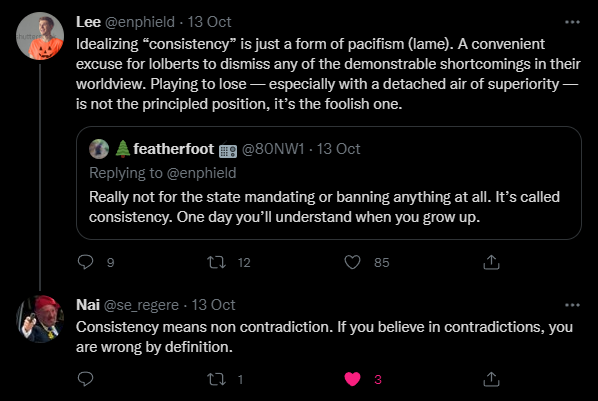
\includegraphics[width=.9\linewidth]{./images/enphield-against-logic.png}
\end{center}

\begin{center}
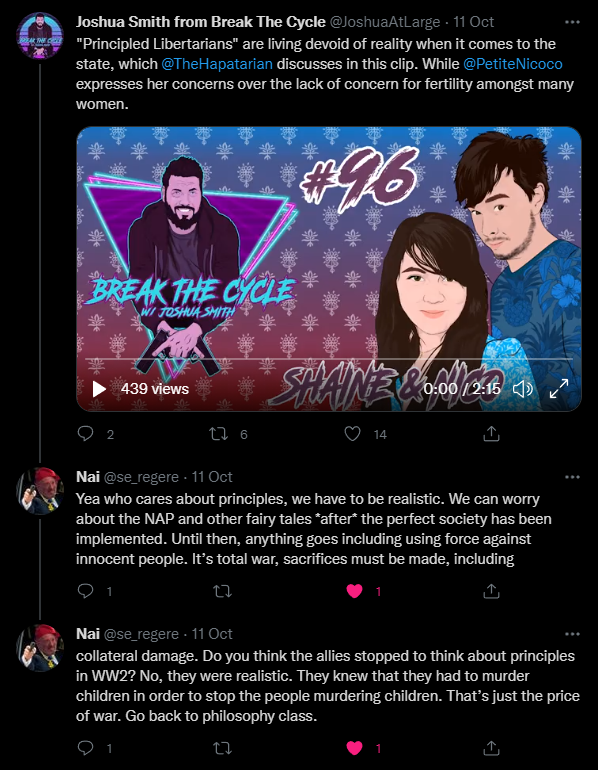
\includegraphics[width=.9\linewidth]{./images/joshuaatlarge-against-logic.png}
\end{center}

\begin{center}

\includegraphics[width=.9\linewidth]{./images/quinones-against-logic.jpg}
\end{center}

\section{We Can Have Freedom After the Revolution}
\label{sec:orgb70973b}
We are fast approaching a time when it will be impossible to catch out neo-prags with reductios ad absurdum. Normally what you would do to show these people that they hold bad beliefs is ask them something along the line of; ``would you kill innocent people to achieve your desired political ends,'' which is met with a resounding ``no'' in any reasonable group of libertarians. But some neo-prags can be seen on twitter advocating that children be slaughtered and that the families of politicians be coerced. I cannot help but recall a story that Michael Malice tells\footnote{\url{https://www.youtube.com/watch?v=XdkjMzYITbI}} of Emma Goldman, a leftist anarchist who was deported from the US to the Soviet Union. Upon arrival she was horrified at the many things Lenin was doing and she confronted him in his office, saying; ``this is not what we are about, the revolution is about freedom''\footnote{I am paraphrasing, watch the clip if you want it from the horses mouth} to which lenin responded that freedom was a bougoise contrivance, and you cannot have it in the midst of a revolution.

\section{Living in Ancapistan in Your Head}
\label{sec:org95d4240}
Living in ancapistan in your head is a common remark by neo-prags, used as a derision of people they see as too principled, saying that they instead live in political reality, and that being an ancap means you rely on a utopian future that either will never happen or will not happen in the ancaps lifetime. I mentioned some examples above, of the mandates and counter-mandates, there is also the borders issue, and sometimes if they are more MAGA aligned they will be upset over social media censorship and want that regulated.

Danny Duchamp has an excellent defense\footnote{see: Danny Duchamp, ``In Defense Of Living In Ancapistan In Your Head,'' \url{https://www.youtube.com/watch?v=sKnVeP7\_xSQ}} of the idea of living in anarcho-capitalism in ones head, which I shall heavily tax here, but you should watch the full thing. It is worth noting right off the bat that Murray Rothbard lived in anarcho-capitalism in his head, so too did most of the greats. Ron Paul hardly acquired the presidency and even if he did, you are naiave if you think he would be able to get anything done with the lengths that the Cathedral went to to stop someone as unlibertarian as Trump. We are diametrically opposed to every form of political power, they will never be our friends, we are forced to live, and to preach anarcho-capitalism in our heads, as this is how we reach the remnant. Further, principles are not just intellectual abstractions that don't apply to your life, you use principles to inform you on how to live ethically in a complicated world. No man has the capacity to understand all the cogs at play, else he could centrally plan, which we don't think is possible. So any man must employ aids to his action, so that he knows when he is being good and when he is being evil.

There is also the snuck premise that living by your principles will just lead to you getting run over by those who don't, and that by abandoning principles you gain far more ground. But this is not at all how politics works. You have a negligible impact on any political issue, whether you live by principles or not. The benefit in living by principles is that you can look yourself in the mirror and know that you are not evil, that you would walk away from omelas, that you would not be the guard at a prison camp.

Duchamp gives an analogy from Physics, that of the Second Law of Thermodynamics. The law states that in any isolated system, entropy cannot decrease, that is to say, that any isolated system will tend to thermodynamic equilibrium. But, in reality we don't see any isolated system, every system we come accross has energy coming in from outside, and/or energy leaving from it. So are physicists ``living in the Second Law of Thermodynamics in their heads?'' Is it pointless to consider the ideal case? Of course not, looking at the ideal case gives you a baseline with which you can analyse the real world with all its messiness. Relating this back to anarcho-capitalism, we could ask whether ancap would devolve into statism, or rather, would we expect it to. This is asking whether private security firms have a tendency towards monopolisation, which any austrian will tell you isn't the case. But that requires us to look at the praxeologic ideal, rather than looking to the real world. Basing economic theory like that on empirical observation is epistemelogically flawed, and I think the neo-prags know this, yet they are basing their ethics on empiricism, surely just as flawed. That is to say, neo-prags can be reasonably framed as ethical-keynesians, not just for their empiricism but for their high-time preference.

\section{Preferences Aren't Laws}
\label{sec:org30097cd}
Neo-prags will often share memes of this sort:
\begin{center}

\includegraphics[width=.9\linewidth]{./images/cant-complain-fries-cold.jpg}
\end{center}

This is an equivocation tactic, they want people to believe, and perhaps they themselves believe, that they are taking up the position this meme takes. Namely, that it is silly to tell people that they are not allowed to complain about the actions of a private company, as this is a rejection of preference. But that is not at all what neo-prags advocate, they wish to violently coerce rather than criticise and peacefully disassociate from companies who do things they dong like. Their frequent uttering of the ``it's a private company bro'' meme is an attempt to conflate principled libertarians with the leftist scourge, which sets a false dichotomy between a principled left and an unprincipleld right. It is very much not a good idea to cede the concept of principle to the left, as that is, as I explained above, ceding the concept of being correct to the left.

\section{I'm Just Shitposting Bro, It's Called Irony}
\label{sec:org741f1aa}
To round off this video, I present a prediction. If everything goes the way I hope it goes and larger names in the space start publicly calling out the neo-prag cancer, I believe they will retreat into ``it's just ironic shitposting, stop taking it so seriously bro.'' Neo-pragmatism can only live in the dark, when large names in the community point out their failings they will be less comfortable in their convictions, and as they have no principle to fall back on, they cannot re-enforce those convictions. This would be the ideal end to the problem, the vanguard could once again get to work at vying for liberty, rather than having to concern themselves with subversion. However, this could just as easily lead to a fragmentation of the movement analogous to the famous Cato vs Mises split. Only time will tell.

\section{Notes}
\label{sec:orgf8c1afe}
\begin{itemize}
\item why did heise start the MC?
\begin{itemize}
\item product of the Ron Paul revolution
\begin{itemize}
\item high energy
\item electric
\item unifying
\item effective
\end{itemize}
\item ``a lot of it is good people but theyve been fed lies'' \url{https://youtu.be/2b01qnZYQJE?t=1851}
\begin{itemize}
\item Pete Quinones
\end{itemize}
\end{itemize}
\item Reach the Remnant \url{https://www.youtube.com/watch?v=EhEAQCsSFfU}
\begin{itemize}
\item be brave rather than sacrificing the message to pander
\item ``what drew me to the mises caucus is that they are focused on principled messaging'' \url{https://youtu.be/EhEAQCsSFfU?t=255}
\end{itemize}
\item Quinones heise interview
\begin{itemize}
\item 1:50 - goal is to get the LP back to strict libertarian principles
\end{itemize}
\end{itemize}
\section{Points to include}
\label{sec:org1324cd6}
Using the state to implement our ends is a deal with the devil

\begin{quote}
You know you are a part of the regime when:

You always understood why your minority political opinions would never be adopted by the majority so you abandon them for authoritarianism out of frustration and high time preference.
 --- @ReadingMises, \url{https://twitter.com/ReadingMises/status/1448936188929249299?s=20}
\end{quote}

\begin{quote}
This is the most urgent problem in intralibertarian discourse. Whether or not it is addressed will determine whether the movement will be characterized by the principles of liberty or \textbf{impulsive reactions against whatever the enemy does}.
\end{quote}
\end{document}
